\documentclass[letter]{article}

\usepackage[margin=2cm]{geometry}
\usepackage{amsmath}
\usepackage{amsfonts}
\usepackage{graphicx}
\usepackage{hyperref}
\usepackage{mathtools}
\usepackage{physics}

\title{Spin Precession in a Magnetic Field}
% Put your name here
\author{Your Name}

% Put the date here
\date{Today}

\begin{document}
\maketitle

In this article, we examine the precession of a spin $\frac{1}{2}$ in a magnetic field.

We consider a magnetic field $\vb{B} = B\vu{z}$. The Hamiltonian is $H = \vb{H} = -\vb{\mu}\vdot\vb{B} = -\gamma\vb{B}\vdot\vb{S}$. For a spin $\frac{1}{2}$, $H = -\frac{\gamma\hbar}{2}\vb{B}\vdot\vb{\sigma}$. Let $\omega = \gamma B$, where $\vb{B} = \vu{n}$. Choosing units such that $\hbar = 1$, we have $H = -\frac{\omega}{2} \vu{n}\vdot\vb{\sigma}$.

We measure time in units of $\frac{1}{\omega}$. Therefore one oscillation corresponds to $t = \pi$. In these units, the Hamiltonian is simply $H = - \vu{n}\vdot\vb{\sigma}$. Choosing the magnetic field to be along the $z$ direction, that is $\vb{B} = B\vu{z}$, the Hamiltonian is $H = -\sigma_z$.

Figure \ref{fig:expsigma} shows the time evolution of the expectation value of the Pauli operators $\sigma_x, \sigma_y, \sigma_z$. As we expect since $\sigma_z$ commutes with the Hamiltonian, the expectation value $\expval{\sigma_z}$ does not change with time. Figure \ref{fig:blochvector} shows a few snapshots in the precession of the spin on the Bloch sphere during one oscillation. As expected we see a clockwise precession of the spin and the Bloch vector.

\begin{figure}
  \centering
  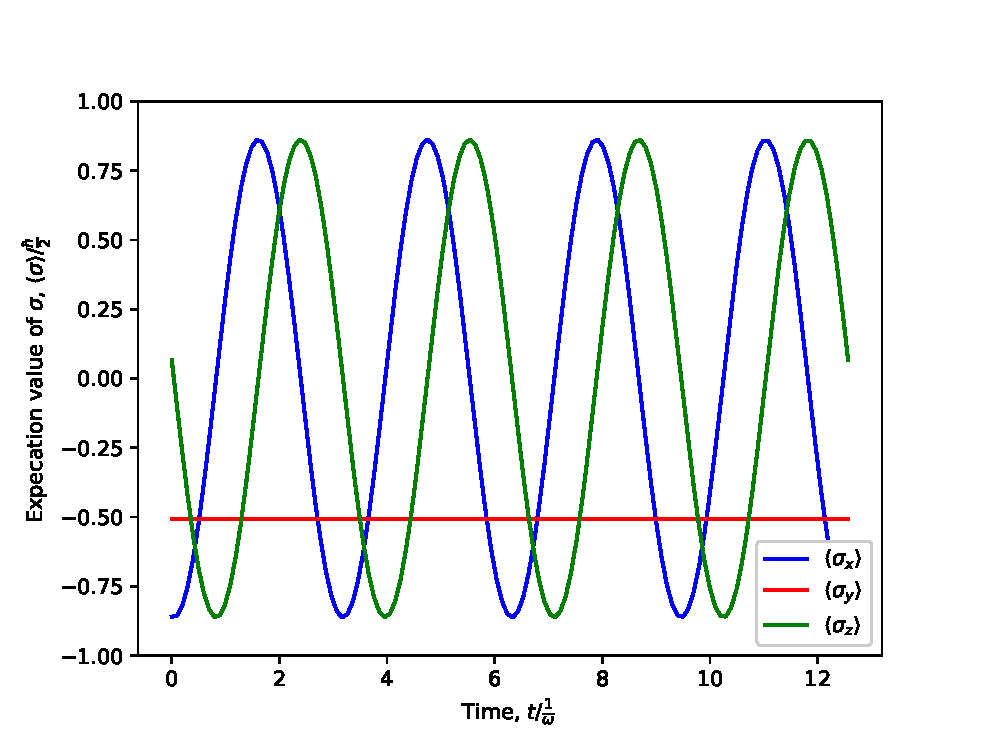
\includegraphics{exp_sigma.eps}
  \caption{The expectation values of the Pauli operators $\expval{\sigma_x}, \expval{\sigma_y}, \expval{\sigma_z}$ under the Hamiltonian as a function of time. Note that the expectation value $\expval{\sigma_z}$ does not change as $\sigma_z$ commutes with the Hamiltonian.}
  \label{fig:expsigma}
\end{figure}



\begin{figure}
  \centering
  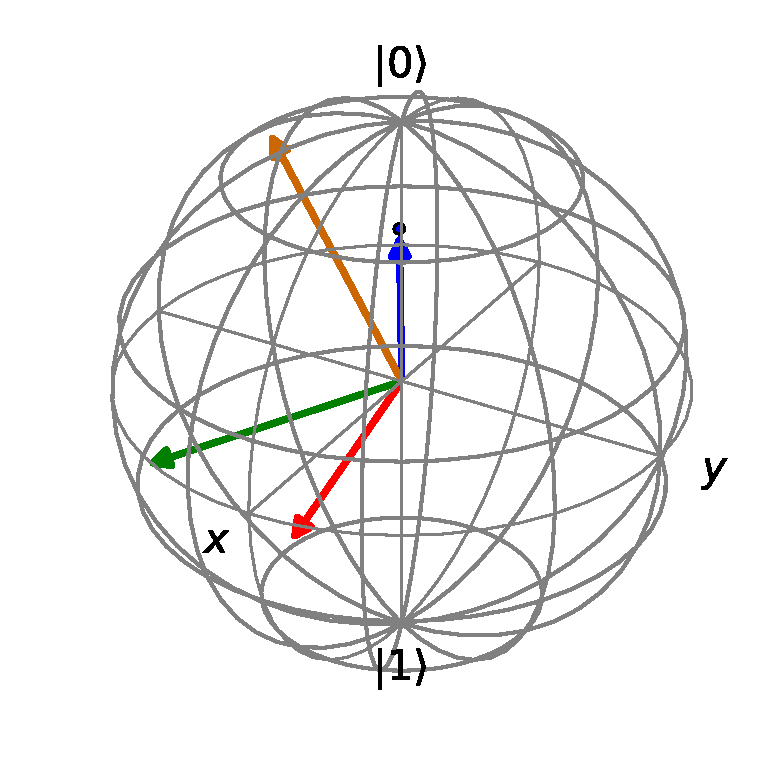
\includegraphics{bloch.eps}
  \caption{The Bloch vector at times $t=0, \frac{\pi}{4}, \frac{\pi}{2}, \frac{3\pi}{2}$, in blue, red, green and brown respectively. The intial Bloch vector is marked with a dot.}
  \label{fig:blochvector}
\end{figure}


\end{document}
